	% !TEX TS-program = XeLaTeX
% use the following command:
% all document files must be coded in UTF-8
\documentclass[portuguese]{textolivre}
% build HTML with: make4ht -e build.lua -c textolivre.cfg -x -u article "fn-in,svg,pic-align"

\journalname{Texto Livre}
\thevolume{18}
%\thenumber{1} % old template
\theyear{2025}
\receiveddate{\DTMdisplaydate{2025}{7}{16}{-1}} % YYYY MM DD
\accepteddate{\DTMdisplaydate{2025}{9}{10}{-1}}
\publisheddate{\DTMdisplaydate{2025}{9}{28}{-1}}
\corrauthor{Monica Aparecida Asquino}
\articledoi{10.1590/1983-3652.2025.60367}
%\articleid{NNNN} % if the article ID is not the last 5 numbers of its DOI, provide it using \articleid{} commmand 
% list of available sesscions in the journal: articles, dossier, reports, essays, reviews, interviews, editorial
\articlesessionname{reports}
\runningauthor{Asquino e Kniess} 
%\editorname{Leonardo Araújo} % old template
\sectioneditorname{Daniervelin Pereira}
\layouteditorname{Leonado Araújo}

\title{Integrando a Internet das Coisas na Robótica Educacional por meio da Abordagem da Aprendizagem Criativa}
\othertitle{Integrating the Internet of Things into Educational Robotics through the Creative Learning Approach}
% if there is a third language title, add here:
%\othertitle{Artikelvorlage zur Einreichung beim Texto Livre Journal}

\author[1]{Monica Aparecida Asquino~\orcid{0009-0001-7768-9059}\thanks{Email: \href{mailto:monica.asquino@gmail.com}{monica.asquino@gmail.com}}}
\author[2]{Janine Kniess ~\orcid{0000-0002-6595-8063}\thanks{Email: \href{mailto:janine.kniess@udesc.br}{janine.kniess@udesc.br}}}
\affil[1]{Escola Municipal Dom Jaime de Barros Câmara, Joinville, SC, Brasil.}
\affil[2]{Universidade do Estado de Santa Catarina, Programa de Pós-Graduação em Computação Aplicada, Joinville, SC, Brasil.}

\addbibresource{article.bib}
% use biber instead of bibtex
% $ biber article

% used to create dummy text for the template file
\definecolor{dark-gray}{gray}{0.35} % color used to display dummy texts
\usepackage{lipsum}
\SetLipsumParListSurrounders{\colorlet{oldcolor}{.}\color{dark-gray}}{\color{oldcolor}}

% used here only to provide the XeLaTeX and BibTeX logos
\usepackage{hologo}

% if you use multirows in a table, include the multirow package
\usepackage{multirow}

% provides sidewaysfigure environment
\usepackage{rotating}

% CUSTOM EPIGRAPH - BEGIN 
%%% https://tex.stackexchange.com/questions/193178/specific-epigraph-style
\usepackage{float}
\usepackage{epigraph}
\usepackage{soulutf8}
\sethlcolor{yellow}

\soulregister\cite7
\soulregister\footnote7

\renewcommand\textflush{flushright}
\makeatletter
\newlength\epitextskip
\pretocmd{\@epitext}{\em}{}{}
\apptocmd{\@epitext}{\em}{}{}
\patchcmd{\epigraph}{\@epitext{#1}\\}{\@epitext{#1}\\[\epitextskip]}{}{}
\makeatother
\setlength\epigraphrule{0pt}
\setlength\epitextskip{0.5ex}
\setlength\epigraphwidth{.7\textwidth}
% CUSTOM EPIGRAPH - END

% LANGUAGE - BEGIN
% ARABIC
% for languages that use special fonts, you must provide the typeface that will be used
% \setotherlanguage{arabic}
% \newfontfamily\arabicfont[Script=Arabic]{Amiri}
% \newfontfamily\arabicfontsf[Script=Arabic]{Amiri}
% \newfontfamily\arabicfonttt[Script=Arabic]{Amiri}
%
% in the article, to add arabic text use: \textlang{arabic}{ ... }
%
% RUSSIAN
% for russian text we also need to define fonts with support for Cyrillic script
% \usepackage{fontspec}
% \setotherlanguage{russian}
% \newfontfamily\cyrillicfont{Times New Roman}
% \newfontfamily\cyrillicfontsf{Times New Roman}[Script=Cyrillic]
% \newfontfamily\cyrillicfonttt{Times New Roman}[Script=Cyrillic]
%
% in the text use \begin{russian} ... \end{russian}
% LANGUAGE - END

% EMOJIS - BEGIN
% to use emoticons in your manuscript
% https://stackoverflow.com/questions/190145/how-to-insert-emoticons-in-latex/57076064
% using font Symbola, which has full support
% the font may be downloaded at:
% https://dn-works.com/ufas/
% add to preamble:
% \newfontfamily\Symbola{Symbola}
% in the text use:
% {\Symbola }
% EMOJIS - END

% LABEL REFERENCE TO DESCRIPTIVE LIST - BEGIN
% reference itens in a descriptive list using their labels instead of numbers
% insert the code below in the preambule:
%\makeatletter
%\let\orgdescriptionlabel\descriptionlabel
%\renewcommand*{\descriptionlabel}[1]{%
%  \let\orglabel\label
%  \let\label\@gobble
%  \phantomsection
%  \edef\@currentlabel{#1\unskip}%
%  \let\label\orglabel
%  \orgdescriptionlabel{#1}%
%}
%\makeatother
%
% in your document, use as illustraded here:
%\begin{description}
%  \item[first\label{itm1}] this is only an example;
%  % ...  add more items
%\end{description}
% LABEL REFERENCE TO DESCRIPTIVE LIST - END


% add line numbers for submission
%\usepackage{lineno}
%\linenumbers

\begin{document}

\maketitle

\begin{polyabstract}

\begin{abstract}
A Robótica Educacional tem sido adotada na prática escolar como forma de engajar os alunos na busca por um aprendizado ativo e interdisciplinar. No entanto, em uma sociedade conectada por meio de redes de computadores, a implementação da Internet das Coisas na Robótica Educacional possibilita uma maior conexão com a realidade fora do ambiente escolar. Este trabalho apresenta o resultado de atividades provenientes da inclusão da Internet das Coisas na Robótica Educacional, desenvolvidas por alunos do ensino fundamental (séries finais) a partir da abordagem da aprendizagem criativa. Como resultado, os alunos apresentaram e executaram projetos envolvendo soluções inovadoras para problemas reais.

\keywords{Robótica \sep Internet das Coisas \sep Aprendizagem Criativa \sep Ensino-Aprendizagem}
\end{abstract}

\begin{english}
\begin{abstract}
Educational Robotics has been adopted in school practice as a way of engaging students in the search for active, interdisciplinary learning. However, in a society connected by computer networks, the implementation of the Internet of Things in Educational Robotics enables a greater connection with reality outside the school environment. This paper presents the results of activities arising from the inclusion of the Internet of Things in Educational Robotics, developed by elementary school students (final grades) using the creative learning approach. As a result, the students presented and executed projects involving innovative solutions to real problems.

\keywords{Robotics \sep Internet of Things \sep Creative Learning \sep Teaching-Learning}

\end{abstract}
\end{english}
% if there is another abstract, insert it here using the same scheme
\end{polyabstract}

\section{Introdução}\label{sec-intro}

As tecnologias digitais estão cada vez mais presentes nas nossas vidas, no modo como nos comunicamos, nos relacionamos e aprendemos. Segundo \textcite {moran}, muitas das formas que estão sendo utilizadas na aprendizagem não correspondem a essa nova realidade na qual nos encontramos. Principalmente ao considerarmos que o ato de educar visa integrar o indivíduo à sociedade na qual está inserido, \textcite [p. 43]{kenski} propõe que ”a educação deve ensinar sobre as tecnologias que estão na base da identidade e da ação do grupo e que se faça uso delas para ensinar as bases dessa educação”.

Visando suprir estas necessidades, o ensino fundamental atual passa por reformulações. Com a introdução de tecnologias digitais e a implementação da Base Nacional Comum Curricular (BNCC). Nesse contexto, novas práticas e abordagens de ensino têm sido aplicadas, discutidas e estudadas para que os alunos da educação básica desenvolvam as novas competências e habilidades propostas. Essas competências visam formar o indivíduo do século XXI.

Uma das práticas que atraem os estudantes e são alvo de muitos estudos é a Robótica Educacional. Essa prática tem sido adotada gradualmente nas últimas décadas como uma abordagem pedagógica interdisciplinar, prática manual e envolvente. A Robótica Educacional tem se tornado uma proposta ativa no ensino de diversas disciplinas. Segundo \textcite{osorio}, a Robótica no ambiente escolar oferece estímulo para o aprendizado por meio de atividades motivadoras nas quais os alunos são levados a resolver situações-problema utilizando o raciocínio lógico e a criatividade, abordando diversas áreas do conhecimento.

Por outro lado, outra prática que tem ganho destaque no cenário educacional é a abordagem da Aprendizagem Criativa. Uma abordagem, que surge na educação para promover o protagonismo do aluno, propondo atividades práticas, multidisciplinares, engajadoras,  partindo do interesse dos estudantes como protagonistas do processo de aprendizagem. Esta abordagem, proveniente do Construcionismo visa uma aprendizagem mais lúdica, criativa e significativa.

Além desses fatores, a própria Base Nacional Comum Curricular (BNCC) tem se concentrado em uma aprendizagem mais ativa e significativa para formar o indivíduo para atuar na realidade em que está inserido, uma realidade extremamente digital. Desse modo, em 2022, com base nas propostas da Sociedade Brasileira da Computação (SBC), foi desenvolvido um complemento visando incluir práticas computacionais no ensino fundamental. Nesse documento, a sexta competência proposta é que o aluno seja capaz de:

\begin{quote}
    Desenvolver projetos, baseados em problemas, desafios e oportunidades que façam sentido ao contexto ou interesse do estudante, de maneira individual e/ou cooperativa, fazendo uso da Computação e suas tecnologias, utilizando conceitos, técnicas e ferramentas computacionais que possibilitem automatizar processos em diversas áreas do conhecimento com base em princípios éticos, democráticos, sustentáveis e solidários, valorizando a diversidade de indivíduos e de grupos sociais, de maneira inclusiva \cite[p. 11]{bncc1}.
\end{quote}

No entanto, o trabalho com a computação no ambiente escolar não é algo tão novo. Em 2017, \textcite {brackmann} já introduzia a importância do pensamento computacional no ambiente escolar. Nesta época seus estudos dividiam o pensamento computacional em quatro pilares básicos: abstração, decomposição, algoritmos e reconhecimento de padrão. No entanto, com o passar dos anos, e a evolução das tecnologias digitais a esses quatro pilares foram acrescentados três: programação, análise e automação \cite {bncc2}. Neste contexto, podemos afirmar que a inclusão de práticas que envolvam a Internet das Coisas (IoT) e a Robótica Educacional em ambiente escolar vem atender a esta ampliação do pensamento computacional, principalmente quando falamos de automação.

Portanto, o objetivo deste artigo é, através de um relato de experiência,  apresentar a prática pedagógica desenvolvida dentro da abordagem da Aprendizagem Criativa, tendo como objeto a criação de projetos inovadores e significativos produzidos por estudantes do ensino fundamental, durante o primeiro semestre de 2024, nas aulas de Robótica Educacional. Para tal, na Seção \ref{sec:fourth} traremos o conceito Aprendizagem Criativa; contextualizando na Seção \ref{sec-normas}, a Robótica Educacional e na Seção \ref{sec:third}, introduziremos o conceito da Internet das Coisas. Apresentaremos a prática desenvolvida na Seção \ref{sec:fifth} e os resultados obtidos na Seção \ref{sec:results}. Por fim, na Seção \ref{sec:seventh}, faremos as considerações sobre a prática.

\section{A Abordagem da aprendizagem criativa na educação}\label{sec:fourth}

A Aprendizagem Criativa é uma abordagem criada a partir do Construcionismo de Seymour Papert. Embora muitos associem o autor à inclusão de práticas computacionais no ambiente escolar, em seus livros o autor propõe  uma aprendizagem mão na massa, significativa e engajadora para todos os envolvidos, seja para construir um castelo de areia, um programa de computador ou uma teoria do universo \cite{papert}.

Neste contexto, o construcionismo propõe que o aluno seja o protagonista de seu aprendizado a partir de criações que lhe sejam significantes. Além disso, esta teoria enfatiza que cada aluno tem o seu modo particular de aprender. Portanto, dentro dessa proposta devemos alterar o foco tradicional do ensino, em que a prática está centrada na didática (o estudo da prática de ensinar), focando, então, na matética (o estudo da prática do aprender). Sendo assim, segundo o construcionismo, é mais importante focar no processo da construção do trabalho do que em seu resultado.

Posteriormente, \textcite{resnick} retoma os estudos acerca do construcionismo, trazendo novas nuances, ampliando suas abordagens e conceitos. A esta nova abordagem, deu-se o nome de Aprendizagem Criativa. Segundo o autor, essa aprendizagem deve ocorrer ao longo da vida, por meio da interação participativa e colaborativa do aluno com suas construções. Essa proposta visa à formação de um indivíduo mais criativo e ativo, capaz de interagir e produzir no mundo em que está inserido.

\begin{quote}
    Vivemos em uma sociedade complexa, com transformações cada vez mais aceleradas e imprevisíveis. Muitas das profissões de hoje não existirão amanhã, e muitas das profissões de amanhã ainda não surgiram. A aprendizagem criativa busca um modelo educacional adequado ao nosso tempo. Um modelo que, inspirado em práticas pedagógicas lúdicas e engajantes para todas as idades, nutra pensadores criativos, pessoas felizes que se sintam confortáveis para enfrentar questões abertas, colaborar com gente diferente e lidar criativamente com recursos ao seu redor \cite [p. 16] {burd}.
\end{quote}

Dentro desta visão, são propostos os chamados “4 Ps da Aprendizagem Criativa”, os quais buscam o protagonismo do estudante na criação de soluções que sejam do seu interesse. Dessa forma, segundo \textcite {resnick}, podemos citar:

\begin{itemize}
\item \textbf{Projeto (Projects):} projetos voltados a solução de problemas reais, identificados pelos alunos, com propósito definido pelo qual o trabalho irá se desenvolver;
\item \textbf{Paixão (Passion):} uma prática que explore os interesses dos alunos;
\item \textbf{Pares (Peers):}  um aprendizado onde os alunos, mediados por seus professores, criem e aprendam o conteúdo através da interação com seus colegas, culminando no compartilhamento; 
\item \textbf{Pensar Brincando (Play):} uma aprendizagem  agradável, divertida, em que é necessária a experimentação para reflexão.
\end{itemize}

Outro fator importante na Aprendizagem Criativa é a espiral criativa. Essa espiral não se trata de uma sequência, mas de passos que devem constar no desenvolvimento do projeto para guiar o aluno por uma experiência criativa. "A espiral de aprendizagem criativa é o motor do pensamento criativo" \cite [p. 12] {resnick}.

Na Figura \ref{figA}, podemos perceber que nessa abordagem o processo de criar está centrado muito mais na imaginação do indivíduo do que na instrução do professor, e que assim o aluno é levado a buscar soluções para problemas que têm sentido para si, e não somente para cumprir determinado conteúdo. A partir do que imagina, o aluno é levado a criar, testar, compartilhar, passando por toda a espiral, uma ou mais vezes. E, ao percorrer essa espiral o aluno será levado a descobrir o conteúdo, que em outros casos seria somente ensinado.

\begin{figure}[htbp]
\centering
\begin{minipage}{.5\textwidth}
 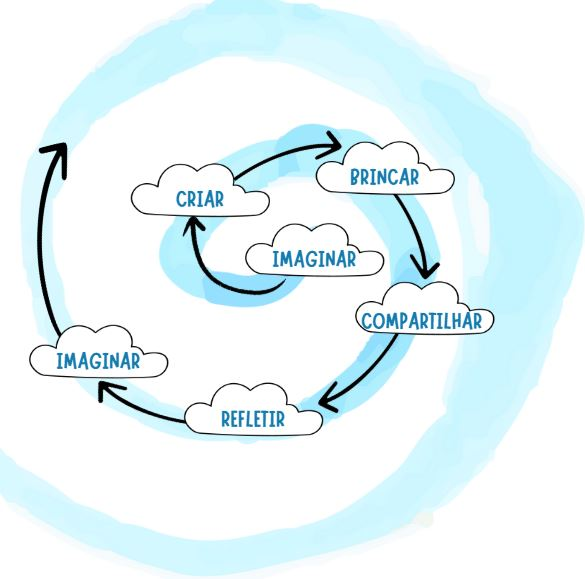
\includegraphics[width=\textwidth]{Figuras/figura01}
 \caption{Espiral da Aprendizagem Criativa.}
  \source{Os autores, baseados em \textcite[p. 40]{resnick}.}
  \label{figA}
\end{minipage}
\end{figure}

Além disso, no construcionismo, propõe-se que as atividades partam do chamado "piso baixo", atividades de fácil execução para que todos possam executar, mas que com "tetos altos", ou seja, que os alunos possam ir além, tanto quanto possível \cite {resnick,papert}. Posteriormente, \textcite {resnick} ampliou este conceito, adicionando as paredes amplas, ou seja, permitir a livre criação por parte dos alunos, segundo seus interesses, abraçando diversas tecnologias, para desenvolver os mais variados projetos, proporcionando a relevância para o aprendizado. “Se os projetos são todos parecidos, sentimos que algo deu errado, ou seja, as paredes não foram amplas o suficiente” \cite [p. 61] {resnick}. 

Nesse sentido, trabalhar com a abordagem da Aprendizagem Criativa significa permitir que os alunos partam do que é significativo para eles para criarem soluções reais para problemas identificados por eles mesmos. Assim, a partir de qualquer proposta, os alunos poderão construir seu conhecimento. No presente projeto, o aprendizado foi baseado em soluções criadas por meio da IoT associada à Robótica Educacional.

\section{Robótica Educacional}\label{sec-normas}

A Robótica Educacional vem ganhando cada vez mais espaço no cotidiano escolar. Trata-se de uma atividade que leva a prática pedagógica para a sala de aula, podendo conceituar situações, sugerir resoluções de problemas ou ainda estimular a criação de algo para a diversão.  

Segundo \textcite{valente}, a Robótica Pedagógica promove atividades de construção, automação e controle de dispositivos robóticos, com aplicações concretas de conceitos, em ambientes de ensino e de aprendizagem, onde o dispositivo robótico é programado para exercer determinadas tarefas, respondendo por meio de reações ao ambiente.

Embora, às vezes, pareça não ter propósito, a criação de algo pelo aluno, essa prática estabelece conexões, exige reflexões matemáticas e de outras disciplinas, requer planejamento e organização para se chegar ao produto final, segundo \textcite {fiorio,teixeira}. A Robótica Educacional promove o aprendizado por meio da criação de projetos que visam à solução de problemas do cotidiano de maneira lúdica. Nesse processo, os alunos trazem a teoria para a prática, abordando várias áreas do conhecimento. Nesse contexto, a Robótica Educacional se mostra uma ferramenta educacional atrativa e estimulante \cite{osorio}. 

\begin{quote}
	Assim, de modo geral, as atividades de robótica pedagógica podem ser vistas como programação, com a vantagem de trabalhar com objetos concretos, como máquinas que se movem como elevadores, máquina de lavar roupa etc., cujo comportamento é produzido pela combinação de conceitos abstratos de diferentes áreas do conhecimento, como Ciências, Matemática; e conhecimentos de Engenharia, como automação, controle de mecanismos eletromecânicos. Todas essas atividades envolvem etapas como concepção, implementação, construção, automação e controle do mecanismo \cite [p. 876] {valente}.
\end{quote}

Dessa maneira, é possível aplicar a Robótica Educacional de diferentes formas, utilizando materiais variados e propondo atividades que vão das mais simples às mais complexas. A proposta pode partir da utilização somente de materiais eletrônicos reciclados, como motores, fios elétricos, componentes de aparelhos antigos, baterias e pilhas, ou até mesmo de aparelhos inteiros que já não são usados. Para gerenciar as tarefas a serem executadas, podem ser utilizados microcontroladores associados a esses elementos. Atualmente, é possível encontrar alguns microcontroladores sendo utilizados para essa função no espaço escolar -- o mais comum entre eles é o Arduíno Uno. Trata-se de uma placa capaz de gerenciar inúmeras funções que utilizem sensores e atuadores, permitindo as mais variadas criações.

No entanto, buscando promover uma robótica mais acessível,  optou-se por trabalhar placa BBC micro:bit\footnote{Disponível em: \url{https://microbit.org/about/}}. Nessa placa, é possível optar por uma programação em blocos (piso baixo) ou JavaScript (teto alto). Além disso, a placa conta com diversos sensores e atuadores já integrados no microcontrolador. Dessa forma, devido a sua praticidade, muitas práticas de robótica já estão migrando seus projetos para o micro:bit. 

Outro fator relevante é que na programação em blocos, como apresentado na Figura \ref{fig-img-a}, os blocos substituem as linhas de código escritas em uma linguagem de programação usual e passam a ter um formato e uma cor específicos, que remetem à função de cada bloco.  A combinação desses blocos para formar uma estrutura com início, processos e resultados forma o programa em blocos \cite{IDCode}. Na Figura \ref{fig-img-a}, apresenta-se um exemplo de comunicação em rádio desenvolvido com a programação em blocos na placa BBC micro:bit.

Essa opção está alinhada à abordagem da Aprendizagem Criativa, na qual o trabalho com essa placa pode ser considerado uma atividade de piso baixo, acessível para todos e que oportuniza aos alunos a possibilidade de ir além, corroborando com o teto alto. Além disso, uma vez que as criações podem ser variadas e aplicadas de diversas maneiras, podemos dizer que temos também o conceito de paredes amplas.


\begin{figure}[h!]
\centering
\begin{minipage}{1\textwidth}
 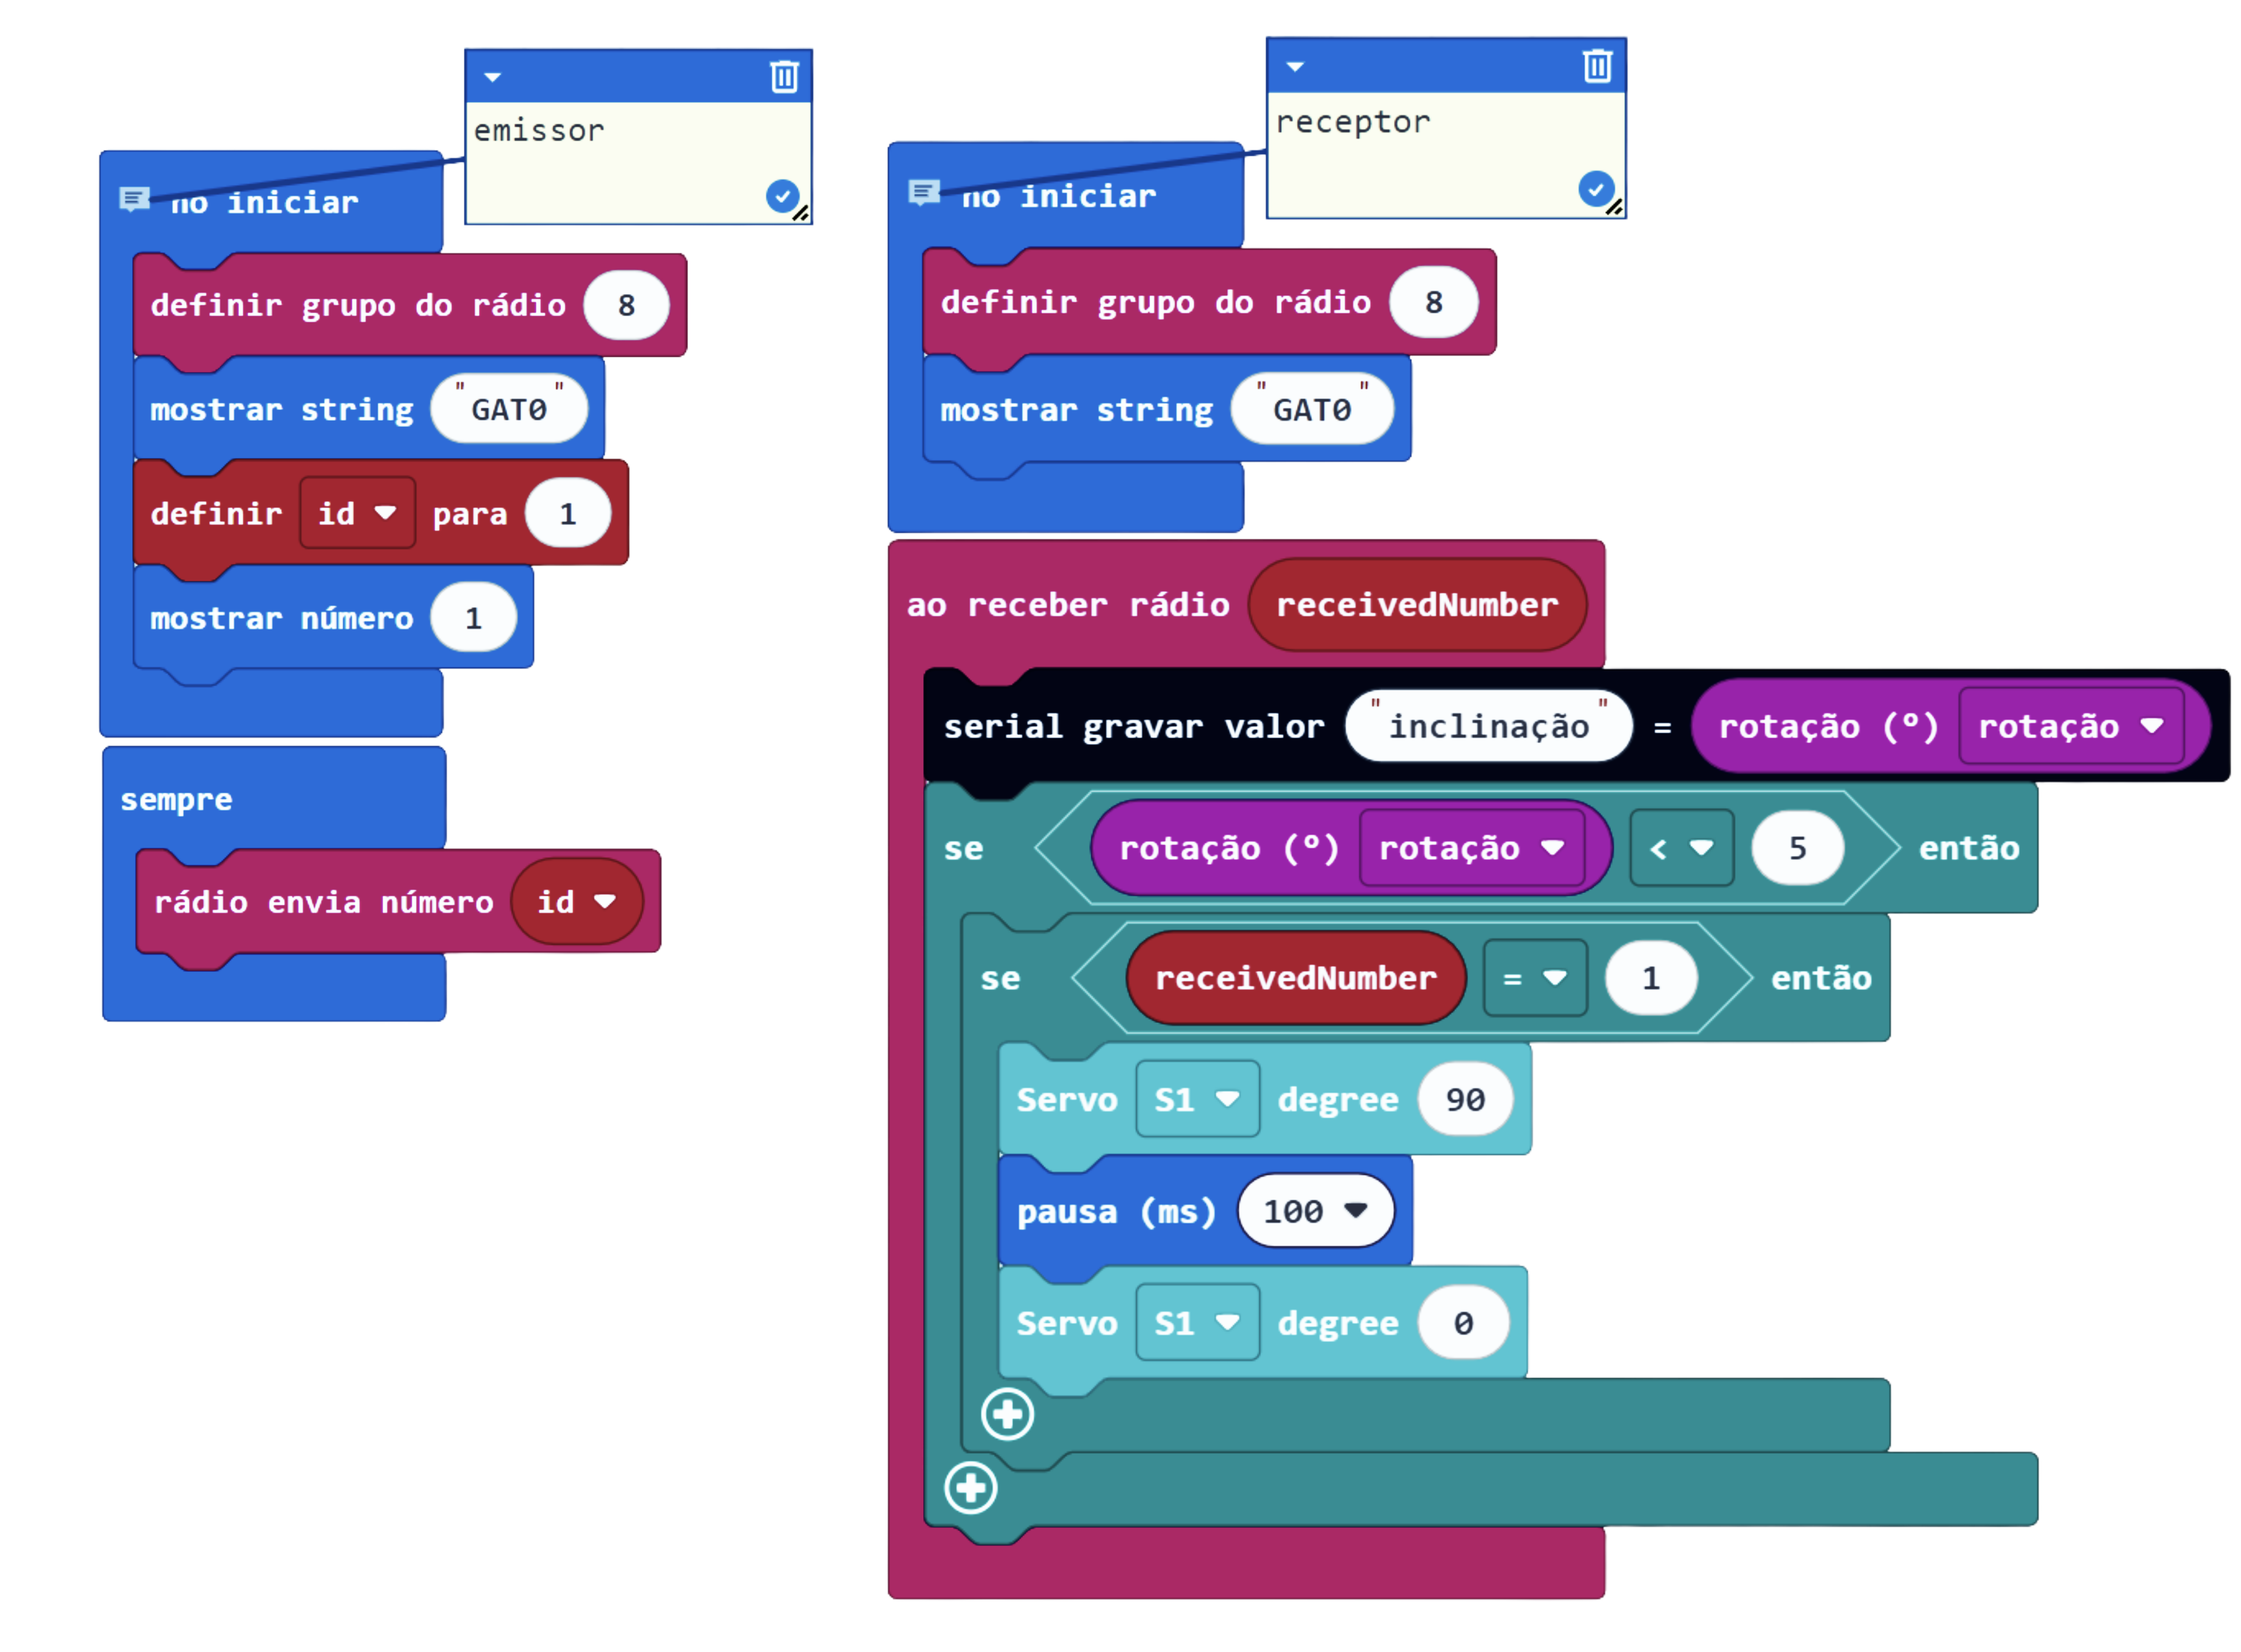
\includegraphics[width=0.87\linewidth, height=0.41\textheight]{Figuras/figura02.png}
 \caption{Programação em Blocos. Exemplo de Comunicação em Rádio no micro:bit.}
 \label{fig-img-a}
 \source{Os autores, 2024.}
\end{minipage}
\end{figure}

Na placa BBC micro:bit, conforme apresentado na Figura \ref{fig-img-microbit}, encontramos diversos atuadores, como uma matriz de LEDs e buzzers. Ela também possui sensores variados, como acelerômetro, sensor de luz, sensor de temperatura, magnetômetro e sensor de toque. Também podemos encontrar botões e pinos de conexão. Outro fator importante é a capacidade de comunicação do micro:bit, que pode ser programado para atuar com Bluetooth ou com comunicação de rádio.

\begin{figure}[H]
\centering
\begin{minipage}{.7\textwidth}
 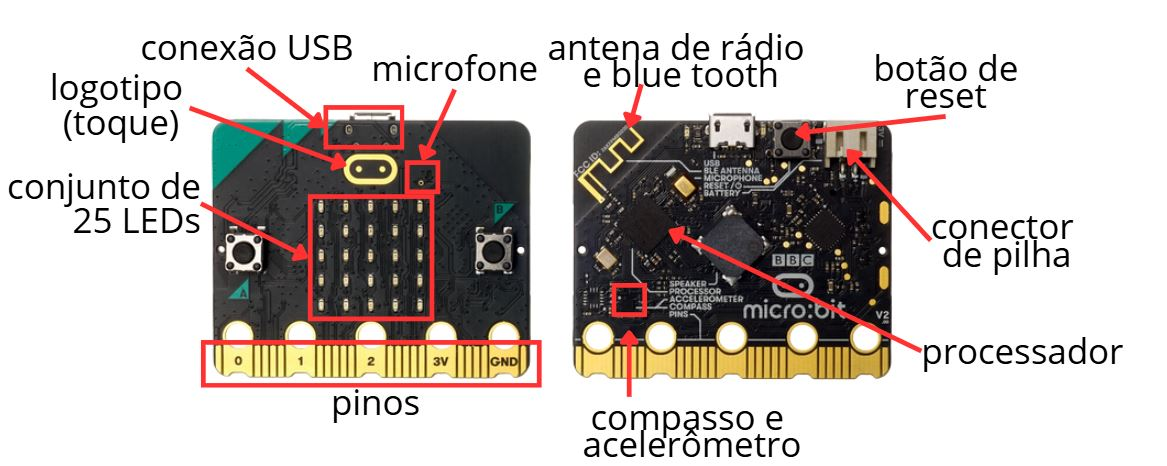
\includegraphics[width=\textwidth]{Figuras/figura03}
 \caption{Recursos da Placa BBC micro:bit.}
 \label{fig-img-microbit}
 \source{Os autores, baseados em \textcite{microbitfoundation}.}
\end{minipage}
\end{figure}

Segundo \textcite {osorio}, o BBC micro:bit é um dispositivo de baixo custo e fácil de usar, além de ser uma ferramenta poderosa, capaz de aprimorar a aprendizagem ao permitir que o aluno aplique a programação para resolver problemas do mundo real por meio de experimentos práticos. Embora o micro:bit seja uma placa com inúmeras funcionalidades e possua pinos nos quais possam ser instalados alguns componentes, ele é um tanto limitado quando utilizado sozinho para finalidades relacionadas à robótica. Portanto, visando oferecer alternativas de piso baixo para os alunos, foi acoplada a ele a extensão da kittenbot\footnote{\url{https://kittenbothk-eng.readthedocs.io/en/latest/microbitv2/intro.html}}, robotbit. Essa extensão permite que os alunos instalem servos, motores e sensores de maneira simples, sem limitar seus projetos. Dessa maneira, ao acoplar a placa BBC micro:bit a esta extensão, ampliamos as possibilidades criativas dos alunos.


Ao trazer a programação e a robótica para a proposta, proporcionou-se aos alunos a exploração de novas aplicações adequadas à realidade de cada um. Buscou-se que essas propostas estivessem mais voltadas às práticas e relacionadas ao mundo fora do ambiente escolar. Aliado ao uso da Robótica Educacional, propôs-se aos alunos a inclusão da IoT como possibilidade de melhorar e ampliar o projeto de cada grupo. Os conceitos de IoT foram previamente apresentados aos alunos, que compreenderam que, por meio dessa tecnologia, os projetos poderiam incluir a comunicação entre dispositivos micro:bits diferentes, bem como a ativação remota de atuadores.


\section{Internet das Coisas}\label{sec:third}

Em paralelo à Robótica Educacional, temos a IoT, que, por sua vez, é o conceito de objetos interconectados e capazes de transmitir informações sobre seu estado e operação.

O termo "Internet das Coisas" foi mencionado pela primeira vez por Kevin Ashton em 1999 \cite{ashton}, durante uma apresentação sobre o uso da tecnologia RFID em um sistema de gestão de suprimentos conectado à internet. Desde então, esse tema tem ganhado destaque, não se limitando apenas ao RFID, mas envolvendo diversos padrões de comunicação, como WiFi \cite{stallings2004ieee}, NFC \cite{Want2011}, \textit{ZigBee} \cite{LIU201475}, \textit{Bluetooth Low Energy} \cite{Hughes2015}, \textit{Long Range Wide Area Network} (LoRaWAN) \cite{FEHRI20181096}, \textit{SigFox} \cite{MEKKI2018}, entre outros. 

A ideia principal da IoT está na presença de objetos interligados e com acesso à internet, que possuem capacidades de processamento e comunicação. Esses elementos podem interagir entre si para alcançar objetivos comuns \cite{Gubbi2013}.

\textcite[p. 19-20]{lemos} define a IoT como:

\begin{quote}
	uma infraestrutura de rede global dinâmica, baseada em protocolos de comunicação em que  “coisas” físicas e virtuais têm identidades, atributos físicos e personalidades virtuais, utilizando interfaces inteligentes e integradas às redes telemáticas. As coisas/objetos tornam-se capazes de interagir e de comunicar entre si e com o meio ambiente por meio do intercâmbio de dados.
\end{quote}

Neste contexto, temos que a IoT permite que haja a conexão entre pessoas, e  uma variedade de objetos do cotidiano destes indivíduos, como sensores, celulares, entre outros, tornando-os capazes de trocar dados entre si; ampliando a capacidade destes elementos. Segundo \textcite{lemos}, essa comunicação entre dois objetos, ou mais, através das redes, independe da distância, podendo ter, ou não seres humanos envolvidos. Portanto, o termo, segundo o autor se refere a objetos reais que em conexão, comunicação e conectividade, com outros objetos,  produzem ações nos mais diversos campos sociais, e que este funcionamento, pode ser considerado inteligente “na medida em que mudam a própria ação e a de outros nessa relação, independentemente de uma ação humana direta” \cite [p. 27]{lemos}.  

A Internet das Coisas tem se mostrado promissora em diversas áreas, como meio ambiente, educação, saúde, transporte e energia, contribuindo para o desenvolvimento de tecnologias e serviços que visam otimizar a eficiência e a qualidade de vida das pessoas. Portanto, segundo \textcite {cremonini}, ao se trabalhar com a  IoT pode-se contribuir no desenvolvimento das habilidades digitais nos alunos, deixando-os aptos para a realidade da sociedade digital, oportunizando a interação de ferramentas comuns no mundo profissional e pessoal, além de desenvolver habilidades de forma colaborativa  e  criativa, promovendo o pensamento crítico e a resolução de problemas. Sendo assim, "a IoT não só facilita o aprendizado, mas também  promove a formação de habilidades digitais que são indispensáveis em uma sociedade na qual a conectividade e a automação estão presentes em diversos setores" \cite [p. 7795]{cremonini}.

Ao analisarmos a robótica sob uma perspectiva mais abrangente, percebemos que os equipamentos robóticos interconectados entre si se enquadram no contexto da Internet das Coisas. Dessa maneira, podemos dizer que a IoT amplia as funcionalidades das aplicações robóticas convencionais, possibilitando o sensoriamento, a execução de ações e o envio de dados para a internet. A adição de diferentes tecnologias de comunicação sem fio aos microcontroladores permite que os estudantes explorem diferentes cenários, aproximando as atividades desenvolvidas no ambiente escolar de aplicações práticas da IoT.

Desta forma, o que antes, nas práticas robóticas, limitava-se ao controle de LEDs, botões e sensores, com a popularização da IoT, os processos podem ser iniciados a distância, a partir da comunicação entre usuários e suas automatizações, ou ainda por uma comunicação máquina a máquina (M2M).

\section{Metodologia} \label{sec:fifth}

Ao falarmos da Robótica Educacional, estamos falando de uma prática que pode ser utilizada para abordar os mais diversos conteúdos, de modo multidisciplinar. Aliado a essa perspectiva, que ao fim do processo há a promoção da construção de um produto final.

Essa prática já é algo que vem sendo explorada em muitas escolas da rede municipal de ensino de Joinville/SC. No entanto, a questão nessa prática, foi de como promover um maior engajamento dos alunos, buscando resolver problemas cotidianos através da robótica. Além disso, procurou-se oportunizar novos conhecimentos acerca das tecnologias digitais presentes fora dos muros escolares, levando a uma reflexão de sua utilização, bem como gerando produções que possam ser consideradas úteis para toda a comunidade escolar.

Dessa maneira, a proposta da atividade visava não somente ao aprendizado da robótica, mas também à contextualização real do que estava sendo aprendido. Nesse sentido, foram trazidas novas situações de uso da tecnologia, com uma nova abordagem. A atividade teve como objetivo proporcionar aos alunos uma vivência prática e novos conhecimentos sobre a tecnologia que já está presente em nosso cotidiano.

Nesse contexto, visando promover uma atividade bem-sucedida e útil, procurou-se introduzir e analisar a inclusão da IoT na prática da Robótica Educacional em uma abordagem da Aprendizagem Criativa. Para isso, as atividades foram desenvolvidas utilizando a placa BBC micro:bit.

A prática ocorreu no primeiro trimestre de 2024. Os alunos participantes consistiam em 16 alunos voluntários, sendo composto esse grupo de nove meninos e sete meninas, provenientes do 7º ano do ensino fundamental séries finais. O projeto ocorreu no contraturno escolar, quando os alunos tinham a livre escolha de participar desta atividade, podendo deixar de comparecer quando quisessem. Para o desenvolvimento das atividades foram feitos encontros semanais que ocorriam durante 1h e 30min.

Logo no primeiro encontro, os alunos tiveram uma breve apresentação do que seria o projeto, sendo compartilhados com eles os objetivos e a proposta. Para orientar os alunos quanto ao desenvolvimento das práticas foram apresentadas  as rubricas para a avaliação do produto final:

\begin{itemize}
\item \textbf{Utilidade:} a proposta desenvolvida é útil para diversas tipos de pessoas ou situações?
\item \textbf{Funcionalidade:} a proposta desempenha corretamente a função para a qual foi desenvolvida?
\item \textbf{Qualidade:} a proposta está bem construída, esteticamente e finalizada? 
\item \textbf{Desenvolvimento:} a proposta foi desenvolvida com a colaboração de todos os integrantes da equipe?
\item \textbf{Aplicação:} a proposta aplicou um ou mais elementos de IoT em seu produto final?
\end{itemize}

Após a explicação inicial, foi solicitado que os alunos se organizassem em grupos de três ou quatro integrantes. Essa escolha partiu do interesse dos próprios alunos, sem a necessidade de intervenção da professora. Dessa forma, os alunos se dividiram em sete grupos, sendo somente dois grupos mistos; os demais foram formados somente por meninos ou por meninas.

Visando desenvolver uma atividade significativa, voltada à realidade e interesse desses alunos (abordando o “P da Paixão” da Aprendizagem Criativa) todas as decisões referentes ao desenvolvimento do projeto partiram dos próprios alunos. Em discussões no grupo, quando necessário, argumentavam aos demais para que a tomada de decisão fosse unânime.

Para introduzir o assunto, foi necessária uma breve explanação sobre o que seria a IoT. Percebeu-se, então, que os alunos não a conheciam, mas também ficou claro o interesse deles pelo assunto. Muitos dos alunos acreditavam que a IoT seria algo de futuro distante. Alguns desconheciam que muitas aplicações já utilizam elementos da IoT. Mesmo se tratando de uma conversa expositiva, os alunos demonstraram muito interesse no assunto.

A discussão para o grande grupo foi aberta após a apresentação. Os alunos se expressaram, demonstrando suas opiniões sobre o que seria a IoT, o que os havia surpreendido e o que havia despertado seu interesse no tema. Entre todos os alunos participantes, somente um demonstrou conhecer um pouco sobre o tema.

Devido ao fato da atividade ocorrer nas aulas de robótica, debatemos de que modo a IoT poderia melhorar nossas criações robóticas, onde cada aluno pode colocar sua opinião. Alguns alunos citaram que seria fazendo “coisas mais úteis do que robô de competição”, outro aluno mencionou que poderiam ser feitas criações para auxiliar as pessoas, havendo até quem mencionou que deixaria as criações mais divertidas.

Após essa reflexão de como a IoT poderia melhorar nossa vida, trazendo facilidades à realidade, foi feito um levantamento individual pelos alunos de situações em que a inclusão da IoT promoveria uma melhoria na qualidade de vida deles. Esta atividade proporcionou o início da espiral criativa, permitindo aos alunos o primeiro passo: o “imaginar”.

Os grupos foram constituídos, e os alunos tiveram a oportunidade de compartilhar com os colegas suas ideias e conexões estabelecidas com a realidade. Neste momento, o grupo pôde em comum acordo decidir uma solução para ser desenvolvida, repetindo o primeiro passo da Aprendizagem Criativa: "o imaginar". O problema selecionado pelo grupo foi novamente revisto e soluções foram apresentadas. Foi orientado que os alunos focassem somente nas soluções que pudessem ser utilizadas na robótica aliada a IoT. Os alunos também puderam fazer pesquisas na internet para estabelecer conexões com o que estavam imaginando e verificar a exequibilidade, a viabilidade e a real necessidade.

Na segunda aula, com os grupos já definidos, retomou-se a discussão sobre o que seria desenvolvido. Um dos grupos optou por mudar a proposta; os demais continuaram com o planejado. Percebeu-se que, nesse segundo momento, alguns alunos haviam inclusive feito pesquisas sobre o que planejavam desenvolver, demonstrando engajamento na atividade, mesmo sem solicitação e fora do ambiente escolar.

Também, nessa segunda aula, deu-se o início ao desenvolvimento de suas criações, enfatizando o objeto a ser automatizado. Ao executarem esta tarefa, houve situações em que o projeto não saía como o planejado, sendo necessária a intervenção da professora, ou ainda a ajuda de um colega de outra equipe, com ideias que solucionassem o problema.

O material inicial utilizado para as construções foi o Kit de Educacional Atto, devido a sua disponibilidade no ambiente escolar e facilidade de montagem, além de ser um material pedagógico. Entretanto, após a sugestão dos alunos de que a adição de outros materiais recicláveis poderia enriquecer o projeto, expandiu-se a inclusão de elementos externos aos kits.

Nas duas aulas seguintes, as criações foram ampliadas, seguindo pela espiral da Aprendizagem Criativa, desta vez na proposta do "brincar". Brincando, os alunos puderam analisar, trocar ideias, solucionar problemas  e testar suas criações. Nesse momento, retornaram ao imaginar, onde puderam pensar nas automatizações a serem implementadas, incluindo motores, luzes, ou quaisquer outros elementos que julgassem necessários.

Tendo o produto em mãos, partiu-se então, na quinta aula, para a inclusão da robótica. Nesse contexto, foi necessário a retomada do conceito de IoT, enfatizando principalmente na comunicação entre as criações. No caso do micro:bit, embora houvesse possibilidades de utilização com Bluetooth, o meio de comunicação utilizado foi o de rádio, por ser o mais simples de implementação, execução, e não interferência entre os projetos.

Essa comunicação rádio da placa micro:bit opera na faixa de frequência de 2.4GHz. A placa possui um alcance típico de até 70 metros em ambientes abertos. No entanto, assim como outros dispositivos de rádio, o alcance pode variar, dependendo das condições do ambiente e da interferência de obstáculos.

Após uma pequena formação sobre a comunicação da IoT, abordando alguns exemplos comuns no nosso cotidiano, os alunos puderam efetuar testes de rádio do micro:bit, desenvolvendo algumas brincadeiras de comunicação entre as placas para compreenderem o funcionamento na prática.

Portanto, tendo o conhecimento da comunicação entre as placas, os alunos refletiram sobre de que modo seriam implantadas nos projetos, além de quais os obstáculos teriam que considerar para prevenir falhas na comunicação. Nessa aula, somente trabalhou-se na programação com a comunicação de rádio entre dois micro:bits, a fim de explorar a potencialidades, compreender o funcionamento e trazer discussões sobre seu papel no projeto final.

Na sexta aula, o que havia sido imaginado pôde ser colocado em prática, fazendo os devidos ajustes, verificando novas alternativas quando necessário, finalizando desta forma o seu produto. O engajamento e a empolgação dos alunos eram tão grandes que desejavam fazer a apresentação do projeto naquele mesmo dia. No entanto, foram planejadas duas apresentações: a primeira para o próprio grupo e outra para toda a escola.

Na sétima aula, foi possível vivenciar na espiral da Aprendizagem Criativa o "compartilhar". Nessa etapa, os alunos compartilharam com os demais colegas seus projetos, ouvindo sugestões, questionamentos e observações sobre sua criação. Desse modo,  puderam refletir sobre o que criaram, de que forma poderiam melhorar a criação e quais ajustes seriam necessários. Sendo assim, foi possível, na última aula, fazer as melhorias e ajustes necessários. Posteriormente, os projetos foram apresentados na escola, no laboratório \textit{maker}, onde as turmas do ensino fundamental dos anos iniciais, com suas professoras, foram convidadas a conhecer os projetos expostos.

Essa última etapa pode promover a integração da escola com os projetos desenvolvidos, a fim de apreciação. Portanto, a ideia era o compartilhamento e diversão daqueles que estavam presentes. Nesse momento, os professores que acompanhavam suas turmas puderam questionar aos alunos sobre o que foi criado, como foi criado e até dar sua colaboração em forma de sugestão. Muitos desses professores enfatizaram a importância das criações dos alunos.

\section{Resultados}\label{sec:results}

Durante esta proposta foram desenvolvidos seis projetos, pensados para solucionar problemas pertencentes ao mundo dos alunos. Embora alguns projetos tivessem ajustes ainda para serem pensados, todos os projetos foram testados e por fim apresentados à comunidade escolar. 

O Grupo 1 desenvolveu um equipamento para alertar sobre a queda de um idoso que mora na casa ao lado de seus parentes. O equipamento deveria ser acoplado ao ombro do idoso. Quando o acelerômetro detecta uma "queda brusca", ele aciona outro equipamento localizado na casa do familiar, emitindo um som alto e sinais de luz. Questionados se não seria mais fácil o equipamento ser acoplado ao pulso do idoso, como um relógio, por exemplo, os alunos explicaram que o braço se movimenta muito, podendo acusar um falso positivo. Além disso, o segundo dispositivo (o receptor) deveria estar ao alcance de muitas pessoas para que qualquer uma pudesse identificar a queda na casa ao lado e prestar os devidos socorros.

Outro produto desenvolvido pelo Grupo 2 foi um robô varredor controlado por controle remoto. Os alunos foram questionados sobre a existência de produtos semelhantes que não demandam controle remoto. No entanto, a equipe justificou que um robô aspirador limpa de forma automática, mas nem sempre essa limpeza é feita com perfeição quando necessário, principalmente em casos específicos, como em caso de "queda de sujeira". Outra preocupação levantada foi a presença de animais de estimação. Dessa forma, o dono do robô poderia controlá-lo remotamente enquanto assiste à televisão, lê um livro ou faz outras coisas.

Pensando nos animais de estimação, algo que todos os integrantes têm em comum, o Grupo 3 desenvolveu um alimentador automático. O diferencial é que esse alimentador libera ração para gatos somente se o gato estiver na frente dele, e ração para cachorros somente para o cachorro. Nesta proposta, cada animal teria um micro:bit instalado em sua coleira. O equipamento analisa a mensagem de rádio recebida e, se for a esperada, libera o alimento.

O Grupo 4 desenvolveu um projeto pensando no próprio ambiente escolar. Ao perceberem que a professora do espaço \textit{maker} gastava tempo indo e voltando para entregar caixas de tablets, chaves e bilhetes em determinadas turmas, eles decidiram propor uma solução. Dessa forma, foi proposta uma criação para automatizar essa tarefa. Os alunos criaram um robô seguidor de linha para ir até o corredor das salas de aula (no mesmo nível que o espaço \textit{maker}) e fazer a entrega. Para isso, a professora deveria selecionar a sala de entrega no robô. O robô, seguindo a linha, passaria pelas salas e verificaria o número programado em outros micro:bits. Quando chegasse ao número desejado, viraria para a sala correta. O protótipo foi desenvolvido, no entanto, os alunos conseguiram fazer a proposta com 50\% de acerto e os testes foram executados em um espaço reduzido, não correspondente à realidade.

No Grupo 5, o projeto se baseou em algo que a professora estava trabalhando, mas propôs uma solução diferenciada. A proposta visava resolver o problema do esquecimento de crianças em automóveis. Nele, um micro:bit ficaria com o responsável e o outro, na cadeira do bebê. Se o sensor de luz acoplado à cadeirinha verificasse uma presença, soaria um alarme e as luzes piscariam para alertar o responsável.

No projeto do Grupo 6, a proposta foi a irrigação automática das plantas de casa. Um dos alunos justificou que, em sua casa, havia somente plantas de plástico, pois sua mãe não sabia regá-las adequadamente. Nele, a umidade do solo de um vaso de plantas seria verificada pelo micro:bit. Quando necessário, um sinal seria enviado para o outro micro:bit, que acionaria o equipamento desenvolvido para que a rega fosse efetuada.

Todos os projetos foram desenvolvidos seguindo a abordagem da Aprendizagem Criativa, permitindo que os alunos imaginassem suas soluções, criassem o projeto imaginado, brincassem com suas criações de modo a testar e verificar na prática suas soluções. Eles também compartilharam seus projetos com os colegas para obter visões externas. Todos os passos foram mediados pela professora do laboratório \textit{maker}, que orientou os alunos para que alcançassem seus objetivos.

Ao longo do projeto, apenas três alunos deixaram de participar. Um deles deixou por motivos pessoais, e os demais relataram ter perdido o interesse em prosseguir. Um desses alunos justificou sua dificuldade em conciliar a robótica com a programação.
Mesmo assim, percebeu-se, até o final do projeto, o engajamento dos alunos em busca de conhecimento fora dos momentos de encontro, inclusive conversando com seus parentes, pesquisando na internet e perguntando aos colegas. A participação dos alunos também foi um aspecto importante a ser observado: houve poucas faltas, a maioria justificada pelos pais.

Para finalizar o projeto, partimos para a avaliação. Ao retornar às rubricas iniciais, solicitamos que os alunos avaliassem seu projeto conforme estabelecido no início. Percebeu-se que, mesmo sendo uma autoavaliação, os alunos foram bastante criteriosos. Acredita-se que, por esta avaliação não "valer nota", eles se permitiram fazer uma avaliação pautada na realidade.

Meses mais tarde, ao participarem do Campeonato de Robótica da Rede municipal, os alunos participantes deste projeto trouxeram o tema IoT dentro do seu Projeto de Inovação da categoria Lego, demonstrando não só que aprenderam com o tema, mas que julgaram importante ao pensarmos em soluções robóticas.

\section{Considerações finais}\label{sec:seventh}

Este artigo apresentou, por meio de um relato de experiência, a criação de soluções a partir da IoT para problemas reais e plausíveis, na perspectiva da abordagem da Aprendizagem Criativa por alunos de uma escola Municipal de Joinville/SC. A motivação dos projetos se dá principalmente pela proposta de atuarem em situações reais, no cotidiano individual, partindo do desejo de solucionar problemas que efetivamente são percebidos na realidade do grupo.

O artigo discutiu a inclusão da Robótica Educacional aliada ao contexto da IoT como prática capaz de abordar diversas habilidades e competências descritas na BNCC. Essa abordagem permite que os estudantes envolvidos vão além das construções básicas e pensem em soluções reais para problemas que ultrapassam os muros escolares. Também foi possível analisar a inclusão da Aprendizagem Criativa no contexto educacional como uma abordagem que promove o protagonismo dos estudantes, trazendo a produção de uma cultura mão na massa, engajadora e pautada na realidade de cada indivíduo, além de estimular o desenvolvimento de projetos no interesse dos envolvidos. 

Concluímos então, com este projeto, que é possível afirmar que a prática de uma Robótica Educacional aliada à proposta da IoT em uma abordagem da Aprendizagem Criativa pode promover a formação de um indivíduo crítico, criativo, capaz de inferir no mundo que o cerca. Desta forma, sugere-se aqui maiores estudos sobre a implementação da IoT como uma forma de complementar a Robótica Educacional, a fim de promover no aprendizado do aluno um sentido em sua realidade; uma aprendizagem significativa. 

Como trabalhos futuros, sugere-se um maior investimento em técnicas qualitativas, como a análise de conteúdo ou a observação participante sistematizada, para aprimorar os resultados da pesquisa.

\printbibliography\label{sec-bib}

%full list: conceptualization,datacuration,formalanalysis,funding,investigation,methodology,projadm,resources,software,supervision,validation,visualization,writing,review
\begin{contributors}[sec-contributors]
\authorcontribution{Monica Aparecida Asquino}[conceptualization,methodology,projadm,writing,review]
\authorcontribution{Janine Kniess}[conceptualization,validation,writing,review]
\end{contributors}

\begin{dataavailability}
\txtdataavailability{nodata} % options: dataavailable, dataonly, databody, datanotav, nodata
\end{dataavailability}

\end{document}
